%!TEX program = pdflatex
\documentclass{tufte-handout}
%\geometry{showframe}% for debugging purposes -- displays the margins

\usepackage{amsmath}

% Set up the images/graphics package
\usepackage{graphicx}
\setkeys{Gin}{width=\linewidth,totalheight=\textheight,keepaspectratio}
\graphicspath{{graphics/}}

\title{Neutrino Oscillations in Vacuum and Matter \thanks{2015 Summer}}
\author[Lei Ma]{Lei Ma}
\date{May 15 2015}  % if the \date{} command is left out, the current date will be used

% The following package makes prettier tables.  We're all about the bling!
\usepackage{booktabs}

% The units package provides nice, non-stacked fractions and better spacing
% for units.
\usepackage{units}

% The fancyvrb package lets us customize the formatting of verbatim
% environments.  We use a slightly smaller font.
\usepackage{fancyvrb}
\fvset{fontsize=\normalsize}

% Small sections of multiple columns
\usepackage{multicol}

% code highlighting
\usepackage{listings}

% \usepackage{minted}
% \usepackage[utf8]{inputenc}
% \usepackage[english]{babel}

% Provides paragraphs of dummy text

% These commands are used to pretty-print LaTeX commands
\newcommand{\doccmd}[1]{\texttt{\textbackslash#1}}% command name -- adds backslash automatically
\newcommand{\docopt}[1]{\ensuremath{\langle}\textrm{\textit{#1}}\ensuremath{\rangle}}% optional command argument
\newcommand{\docarg}[1]{\textrm{\textit{#1}}}% (required) command argument
\newenvironment{docspec}{\begin{quote}\noindent}{\end{quote}}% command specification environment
\newcommand{\docenv}[1]{\textsf{#1}}% environment name
\newcommand{\docpkg}[1]{\texttt{#1}}% package name
\newcommand{\doccls}[1]{\texttt{#1}}% document class name
\newcommand{\docclsopt}[1]{\texttt{#1}}% document class option name



% For quantum braket notation
\newcommand{\bra}[1]{\left\langle #1\right|}
\newcommand{\ket}[1]{\left| #1\right\rangle}
\newcommand{\braket}[2]{\langle #1 \mid #2 \rangle}
\newcommand{\avg}[1]{\left< #1 \right>}

\begin{document}

\maketitle% this prints the handout title, author, and date

\begin{abstract}
\noindent Notes for neutrino oscillations in vacuum and dense matter.
\end{abstract}



Some symbols and definitions:
\begin{itemize}
\item 
$\Delta = \sqrt{2} G_F n(x) $
\item
$\omega = \frac{\Delta m^2}{2E}$
\end{itemize}




\section{Vacuum Oscillations}

Schrodinger equation is

\begin{equation}
i\partial_t \ket{\Psi} = \mathbf H \ket{\Psi},
\end{equation}

where for relativistic neutrinos, the energy is\footnote{They all have the same momentum but different mass. The thing is we assume they have the same velocity since the mass is very small. To have an idea of the velocity difference, I can calculate the distance travelled by another neutrino in the frame of one neutrino.\newline
Assuming the mass of a neutrino is 1eV with energy 10MeV, we will get a speed of $1-10^{-14}$c. This $10^{-14}$c will make a difference about $3\mathrm{\mu m}$ in 1s.
\newline {\bf To Be Discussed!} \newline Will decoherence happen due to this? }

\begin{align*}
\mathbf H^m &= \begin{pmatrix}\sqrt{p^2 + m_1^2} & 0 & 0 \\ 0& \sqrt{p^2 + m_2^2} & 0 \\ 0 & 0 & \sqrt{p^2 + m_3^2}  \end{pmatrix},
\end{align*}

in which the energy terms are simplified using the relativistic condition

\begin{align}
\sqrt{p^2+m_i^2} & = p\sqrt{1 + \frac{m_i^2}{p^2}} \\
&\approx  p(1 + \frac{1}{2} \frac{m_i^2}{p^2}).
\end{align}


In general the flavor eigenstates are the mixing of the mass eigenstates with a unitary matrix $\mathbf U$, that is

\begin{equation}
\ket{\nu_{\alpha}} =  U_{\alpha i} \ket{\nu_i},
\end{equation}

where the $\alpha$s are indices for flavor states while the $i$s are indices for mass eigenstates.

To find out the equation of motion for flavor states, plugin in the initary tranformation,

\begin{equation}
i  U_{\alpha i} \partial_t \ket{\nu_i} =  U_{\alpha i}  H^m_{ij} \ket{\nu_j}.
\end{equation}

I use index ${}^m$ for representation of Hamiltonian in mass eigenstates. Applying the unitary condition of the transformation,

\begin{equation}
\mathbf I = \mathbf {U^\dagger} \mathbf U,
\end{equation}

I get

\begin{equation}
i U_{\alpha i} \partial_t \ket{\nu_i} =  U_{\alpha i} H^m_{i j}  {U^\dagger_{j\beta}}  U_{\beta k} \ket{\nu_k},
\end{equation}

which is simplified to

\begin{equation}
i \partial_t \ket{\nu_\alpha} = H^f_{\alpha \beta} \ket{\nu_{\beta}},
\end{equation}

since the transformation is time independent.

The new Hamiltonian in the representations of flavor eigenstates reads

\begin{equation}
H^f_{\alpha\beta}  = U^\dagger_{\alpha i} H^m_{ij} U_{j\beta}.
\end{equation}



\subsection{Survival Probability}


The neutrino states at any time can be written as

\begin{equation}
\ket{\Psi(t)}  = X_1 \ket{\nu_1 } e^{-i E_1 t}+ X_2 \ket{ \nu_2 } e^{-i E_2 t},
\end{equation}

where $X_1$ and $X_2$ are the initial conditions which are determined using the neutrino initial states.

Survival probalility is the squrare of the projection on an flavor eigenstate,

\begin{equation}
P_{\alpha}(t) = \lvert \braket{\nu_{\alpha}}{\Psi(t)} \rvert^2.
\end{equation}

The calculation of this expression requires our knowledge of the relation between mass eigenstates and flavor eigenstates which we have already found out.

Recall that the transformation between flavor and mass states is

\begin{equation}
\ket{\nu_i} = U^{-1}_{i\alpha} \ket{\nu_\alpha},
\end{equation}

which leads to the inner product of mass eigenstates and flavor eigenstates,

\begin{align}
\braket{\nu_\alpha}{\nu_i} &= \bra{\nu_\alpha} U^{-1}_{i\beta} \ket{\nu_\beta} \\
& = U^{-1}_{i\beta}\delta_{\alpha\beta} \\
7 = U^{-1}_{i\alpha}.
\end{align}


The survival probability becomes

\begin{align*}
P_\alpha (t) &= \lvert \braket{\nu_\alpha}{ X_1 \ket{\nu_1 } e^{-i E_1 t} X_2 \ket{ \nu_2 } e^{-i E_2 t} }  \rvert^2 \\
& = \lvert  X_1 e^{-i E_1 t} \braket{\nu_\alpha}{\ket{\nu_1} } + X_2 e^{-i E_2 t} \braket{ \nu_\alpha }{ \nu_2 } \rvert^2 \\
& = \lvert \sum_i X_i e^{-i E_i t} U^{-1}_{i \alpha}  \rvert ^2 \\
& = \sum_i X_1^* e^{iE_i t} U^{\dagger *}_{i\alpha} \sum_i X_i e^{-i E_i t} U^\dagger_{i \alpha} \\
& = \lvert X_1 \rvert^2 U^{\dagger *}_{1\alpha} U^\dagger_{1\alpha} + \lvert X_2 \rvert^2 U^{\dagger *}_{2\alpha} U^\dagger_{2\alpha}  + X_1^* X_2 U^{\dagger *}_{1\alpha} U^\dagger_{2\alpha} e^{i E_1 t - i E_2 t} + X_2^* X_1 U^{\dagger *}_{2\alpha} U^\dagger_{1\alpha} e^{i E_2 t - i E_1 t}
\end{align*}


$U^{\dagger *}_{i\alpha}$ stands for the $i$th row and the $\alpha$th column of the matrix $U^{\dagger *}$. 



\subsection{Two Flavor States}


For 2 flavor neutrinos the Hamiltonian in the representation of propagation states,

\begin{equation*}
\mathbf H  = \begin{pmatrix}
E_1 & 0 \\
0 & E_2
\end{pmatrix} 
 = \begin{pmatrix}
p_1 + \frac{1}{2}\frac{m_1^2}{p_1} & 0 \\
0 & p_2 + \frac{1}{2}\frac{m_1^2}{p_2}
\end{pmatrix}.
\end{equation*}

The equation of motion in matrix form is

\begin{equation}
i\partial_t \begin{pmatrix}
\nu_1 \\ \nu_2 \end{pmatrix} = \begin{pmatrix}
p_1 + \frac{1}{2}\frac{m_1^2}{p_1} & 0 \\
0 & p_2 + \frac{1}{2}\frac{m_1^2}{p_2}
\end{pmatrix} \begin{pmatrix}
\nu_1 \\ \nu_2 \end{pmatrix} 
\end{equation}

The flavor eigenstate is a mixing of the propagation eigenstates,

\begin{equation}
\begin{pmatrix}
\nu_a \\ \nu_b \end{pmatrix} = 
\begin{pmatrix} \cos\theta_v & \sin\theta_v \\ -\sin\theta_v  & \cos\theta_v
\end{pmatrix} \begin{pmatrix}  \nu_1 \\ \nu_2
\end{pmatrix}
\end{equation}


Denote the rotation matrix using $\mathbf U$, the transofmation can be written as

\begin{equation}
\ket{\nu_{\alpha}} = \mathbf U_{\alpha i} \ket{\nu_i},
\end{equation}

where $\alpha$ is for the flavor eigenstates and $i$ is for the mass eigenstates.

The survival probability has been derived in previous section, which is the projection of propagation states onto flavor states.

For arbitary initial condition,

\begin{align}
    \Psi(t=0)= A \ket{\nu_a} + B \ket{\nu_b}, 
\end{align}

which can be rewritten into a matrix form,

\begin{align}
    \Psi(t=0) = \begin{pmatrix}
    A & B 
\end{pmatrix}\begin{pmatrix}
    \nu_a \\
    \nu_b 
\end{pmatrix}
\end{align}



To write down the projection, the relation

\begin{align}
    \begin{pmatrix}
        \nu_a \\
        \nu_b
    \end{pmatrix} = \begin{pmatrix}
        \cos\theta_v & \sin\theta_v \\ -\sin\theta_v  & \cos\theta_v
\end{pmatrix} \begin{pmatrix}  \nu_1 \\ \nu_2
\end{pmatrix}
\end{align}

is needed. BTW, the inverse transformation is the transpose of $\mathbf U$ since $\mathbf U$ is unitary, thus we have the relation,

\begin{align}
\begin{pmatrix}
    \nu_1 \\
    \nu_2
\end{pmatrix} = \begin{pmatrix}
\cos\theta_v & -\sin\theta_v \\
\sin\theta_v & \cos\theta_v
\end{pmatrix} \begin{pmatrix}
    \nu_a \\
    \nu_b
\end{pmatrix}
\end{align}

Thus in the state can be written as

\begin{align}
    \Psi(t=0) = \begin{pmatrix}
        A & B 
    \end{pmatrix} \begin{pmatrix}
        \cos\theta_v & \sin\theta_v \\
        -\sin\theta_v & \cos\theta_v 
    \end{pmatrix}\begin{pmatrix}
        \nu_1 \\
        \nu_2
    \end{pmatrix}.
\end{align}

At any $t$, the state is

\begin{align}
    \Psi(t) &= \begin{pmatrix}
        A \cos\theta_v - B \sin\theta_v & A\sin\theta_v + B \cos\theta_v
    \end{pmatrix} \begin{pmatrix}
        \nu_1 e^{-i E_1 t}\\
        \nu_2 e^{-i E_2 t}
    \end{pmatrix} \\
    & = \begin{pmatrix}
        (A \cos\theta_v - B \sin\theta_v) e^{-iE_1 t} & (A\sin\theta_v + B \cos\theta_v
        ) e^{-iE_2t}\end{pmatrix} \begin{pmatrix}
        \nu_1 \\
        \nu_2
    \end{pmatrix}
\end{align}

The survival probability which is projection on a flavor state is written as

\begin{equation}
    P(\nu_\alpha,t) = \lvert \braket{\nu_\alpha}{\Psi(t)} \rvert^2.
\end{equation}

The survival amplitude for $\nu_a$ is

\begin{align*}
    &\phantom{=}\braket{\nu_a}{\Psi(t)} \\
     =& \bra{\nu_a}\left(  ( A \cos\theta_v - B \sin\theta_v) e^{-iE_1 t} \ket{\nu_1} +  (A\sin\theta_v + B \cos\theta_v
    ) e^{-i E_2t} \ket{\nu_2} \right) \\
     =& \left ( \cos\theta_v \bra{\nu_1} + \sin\theta_v \bra{\nu_2} \right)  \left(   ( A \cos\theta_v - B \sin\theta_v) e^{-iE_1 t} \ket{\nu_1} +  (A\sin\theta_v + B \cos\theta_v
    ) e^{-i E_2 t} \ket{\nu_2}  \right )
\end{align*}

This is simple since the transformation matrix is real.

Applying the condition that the propagation eigenstates are orthonormal, the survival probability is

\begin{align*}
    P(\nu_a,t) & = \lvert \braket{\nu_a}{\Psi(t)}\rvert^2 \\
    & = \lvert \cos\theta_v (A\cos\theta_v -B\sin\theta_v) e^{-iE_1t} + \sin\theta_v(A\sin\theta_v + B \cos\theta_v) e^{-iE_2t} \rvert^2\\
    & =\lvert ( A \cos^2\theta_v - B \sin\theta_v \cos\theta_v ) e^{-iE_1t} + ( A \sin^2\theta_v + B \sin\theta_v \cos\theta_v )e^{-iE_2t} \rvert^2
\end{align*}

In a special limit that $E_1=E_2=E$, the probability becomes

\begin{equation}
    P(\nu_a,t) = \lvert A\rvert^2 
\end{equation}

which is the same as initial probability since there is no mixing at all.

There are two kinds of initial conditions.

\begin{itemize}
    \item
    The neutrinos are all in $\nu_a$ state initially, which means $A=1, B=0$. The survival probability simplifies to
    \begin{align*}
    P(\nu_a,t) & = \lvert \cos^2\theta_v e^{-iE_1t} + \sin^2\theta_v e^{-iE_2t} \rvert^2  \\
    & = \lvert \cos^2\theta_v e^{-i(E_1 - E_2) t} + \sin^2\theta_v \rvert^2
    \end{align*}
    
    As we have already discussed, $E_1-E_2 = \frac{m_1^2 - m_2^2}{2p}$ assuming the neutrinos have the same momentum. \footnote{And here is a question.} Using the notation $\Delta \, m^2 = m_1^2 - m_2^2$ and the approximation that $E\approx p$, the survival probability can be rewritten as
    \begin{align*}
    P(\nu_a,t) & = \cos^4\theta_v + \sin^4\theta_v + \cos^2\theta_v \sin^2\theta_v \left( e^{-i \Delta m^2 t/E} + e^{i \Delta m^2 t/E} \right) \\
    & = 1 - 2\cos^2\theta_v \sin^2\theta_v + 2\cos^2\theta_v \sin^2\theta_v \cos\left( \frac{\Delta m^2 t}{2E}\right) \\
    & = 1 - 2\cos^2\theta_v \sin^2\theta_v \left( 1 - \cos\left( \frac{\Delta m^2 t}{2E} \right)  \right) \\
    & = 1 - 4 \cos^2\theta_v \sin^2\theta_v \sin^2 \left( \frac{\Delta m^2 t}{4E} \right) \\
    & = 1 - \sin^2(2\theta_v) \sin^2 \left( \frac{\Delta m^2 t}{4E} \right)
    \end{align*}
    
    
We always assuming that in the region of interest, all neutrinos are travelling with the same speed, i.e., the speed of light $c=1$. \footnote{which is not true obviously} Time is related to distance, $L = t$. Survival probability at distance $L$ is

\begin{equation}
P(\nu_a, L) = 1 -  \sin^2 (2\theta_v) \sin^2 \left( \frac{\Delta m^2 L}{4E} \right)
\end{equation}
    
    \item
    The neutrinos are all in $\nu_b$ state initially. Equivalently, we have $A=0, B = 1$. Survival probability is
    
    \begin{align*}
    P(\nu_a,t) & = \lvert -\sin\theta_v \cos\theta_v e^{-iE_1t} + \sin\theta_v \cos\theta_v e^{-iE_2t}  \rvert^2 \\
    & = \sin^2\theta_v \cos^2\theta_v \lvert e^{-i(E_1 - E_2)t} - 1 \rvert^2 \\
    & = \sin^2\theta_v \cos^2\theta_v \left(  1 +1 - e^{-i \Delta m^2 t/2E} -  e^{i \Delta m^2 t/2E}  \right) \\
    & = 2 \sin^2\theta_v \cos^2\theta_v \left( 1- \cos\left( \frac{\Delta m^2 t}{2E} \right) \right) \\
    & = \sin^2 ( 2\theta_v ) \sin^2\left( \frac{\Delta m^2 t}{4E}  \right) \\
    &  = \sin^2 ( 2\theta_v ) \sin^2\left( \frac{\Delta m^2 L}{4E}  \right)
    \end{align*}
    
\end{itemize}


\subsection{Density Matrix}

This problem can be solved using density matrix $\rho$ and Von Neumann equation

\begin{equation}
i \partial_t \rho = [H,\rho].
\end{equation}


The initial condition for this equation is

\begin{align*}
\rho(t=0) &= (A \ket{\nu_a} + B \ket{\nu_b} )(A^* \bra{\nu_a} + B^* \bra{\nu_b} ) \\
& = A A^* \ket{\nu_a}\bra{\nu_a} + B B^* \ket{\nu_b}\bra{\nu_b} + A B^* \ket{\nu_a}\bra{\nu_b} + A^* B \ket{\nu_b} \bra{\nu_a} .
\end{align*}

To calculate the propagation of the states, we need the Hamiltonian matrix in flavor basis.

This can be done by finding out how the Hamiltonian matrix transforms from one basis to another.

Using propagation basis,

\begin{equation}
i\partial_t \ket{\Psi_p} = H_p \ket{\Psi_p}.
\end{equation}

The states are $\ket{\Psi} = \mathbf{U} \ket{\Psi_p} $ in flavor basis, which means we could plug in $\ket{\Psi_p} = \mathbf{U^T}\ket{\Psi}$.

\begin{equation*}
i\partial_t \mathbf{U^T} \ket{\Psi} = H_p \mathbf{U^T} \ket{\Psi}.
\end{equation*}

Since $\mathbf{U}\mathbf{U^T}=\mathbf{I}$, we have a clean result by multiplying through the equation by $\mathbf{U}$.

\begin{equation*}
i\partial_t \ket{\Psi} = \mathbf{U} H_p \mathbf{U^T} \ket{\Psi}.
\end{equation*}

So we define $H = \mathbf{U}H_p \mathbf{U^T}$ as the Hamiltonian matrix in flavor basis, which is


\begin{equation}
H = \left(p + \frac{m_1^2+m_2^2}{4p} \right)\mathbf I - \frac{1}{4p}\begin{pmatrix} - \Delta m^2 \cos 2\theta & \Delta^2 m \sin 2\theta \\  \Delta m^2 \sin 2\theta & \Delta^2 m\cos 2\theta \end{pmatrix}.
\end{equation}

The derivation of this is

\begin{align*}
\mathbf H_{\alpha} & = \mathbf U \hat H_j  \mathbf U^T \\
& =  \begin{pmatrix}  \cos\theta & \sin\theta \\ -\sin\theta  & \cos\theta \end{pmatrix} \left( p \mathbf I + \frac{1}{2p}\begin{pmatrix} m_1^2 & 0 \\ 0 & m_2^2 \end{pmatrix} \right)   \begin{pmatrix}  \cos\theta & -\sin\theta \\ \sin\theta & \cos\theta \end{pmatrix} \\
& = p \mathbf I + \frac{1}{2p} \begin{pmatrix} \cos^2\theta m_1^2 + \sin^2\theta m_2^2 & -\sin\theta\cos\theta m_1^2 + \sin\theta\cos\theta m_2^2 \\ -\sin\theta\cos\theta m_1^2 + \sin\theta\cos\theta m_2^2 & \sin^2\theta m_1^2 + \cos^2\theta m_2^2 \end{pmatrix} \\
& = p \mathbf I + \frac{1}{2p} \begin{pmatrix} m_1^2 - \delta^2 m \sin^2\theta & -\frac{1}{2}\sin 2\theta  \delta m^2  \\ -\frac{1}{2}\sin 2\theta  \delta m^2  & m_2^2+ \delta m^2 \sin^2\theta \end{pmatrix} \\
& = p \mathbf I + \frac{1}{2p} \left( \frac{1}{2}(m_1^2+m_2^2) \mathbf I -   \frac{1}{2}\begin{pmatrix} - \delta m^2 \cos 2\theta & \delta^2 m \sin 2\theta \\  \delta m^2 \sin 2\theta & \delta^2 m\cos 2\theta \end{pmatrix} \right) \\
& = \left(p + \frac{m_1^2+m_2^2}{4p} \right)\mathbf I - \frac{1}{4p}\begin{pmatrix} - \delta m^2 \cos 2\theta & \delta^2 m \sin 2\theta \\  \delta m^2 \sin 2\theta & \delta^2 m\cos 2\theta \end{pmatrix}
\end{align*}

Since identity matrix only shifts the eigenvalues we are only interested in the second term, thus the Hamiltonian we are going to use is

\begin{equation}
H = \frac{\Delta m^2}{4E} \begin{pmatrix}
\cos 2\theta &  -  \sin 2\theta \\  - \sin 2\theta & - \cos 2\theta
\end{pmatrix}.
\end{equation}

The equation of motion becomes

\begin{equation}
i \partial_t \begin{pmatrix}
u(t) \\ v(t)
\end{pmatrix} = \frac{\Delta m^2}{4E} \begin{pmatrix}
\cos 2\theta &  -  \sin 2\theta \\  - \sin 2\theta & - \cos 2\theta
\end{pmatrix} \begin{pmatrix}
u(t) \\ v(t)
\end{pmatrix}
\end{equation}

To solve this we need the eigenvalues and eigenvectors of the Hamiltonian matrix.



\subsection{An Example of Survival Probability}

Suppose the neutrinos are prepared in electron flavor initially, the survival probability of electron flavor neutrinos is calculated using the result I get previously.

Electron neutrinos are the lighter ones, then I have ${}_a = {}_e$ and denote ${}_b={}_x$. \footnote{In the small mixing angle limit, 
\begin{equation*}
\begin{pmatrix}\nu_e \\ \nu_x\end{pmatrix} \to \begin{pmatrix}  1 & \theta \\ -\theta  & 1 \end{pmatrix}   \begin{pmatrix}\nu_1 \\ \nu_2\end{pmatrix}
\end{equation*}

which is very close to an identity matrix. This implies that electron neutrino is more like mass eigenstate  $\nu_1$ . By $\nu_1$ we mean the state with energy  $\frac{ \delta m^2 }{4E}$ in vacuum.
}

The survival probability for electron neutrinos is

\begin{align*}
P(\nu_e,L) &= 1-\sin^2(2\theta_v)\sin^2\left( \frac{\Delta m^2 L}{4E} \right) .
\end{align*}






\subsection{Numerical Results for 2 Flavor Oscillations}


To solve a set of first order differential equations, I need the determinant of coefficient matrix. For 2 flavor neutrino oscillations,

\begin{equation*}
\partial_t \begin{pmatrix}
u(t) \\ v(t)
\end{pmatrix} = - i \frac{\Delta m^2}{4E} \begin{pmatrix}
\cos 2\theta &  -  \sin 2\theta \\  - \sin 2\theta & - \cos 2\theta
\end{pmatrix} \begin{pmatrix}
u(t) \\ v(t)
\end{pmatrix}.
\end{equation*}

To find the solutions I need the eigenvalues $\lambda$ I need to find the determinant

\begin{align*}
&\det \left( - i\frac{\Delta m^2}{4E} \begin{pmatrix}
\cos 2\theta &  -  \sin 2\theta \\  - \sin 2\theta & - \cos 2\theta
\end{pmatrix} - \lambda \mathbf{I} \right) \\
=& \begin{vmatrix}
-i \frac{\Delta m^2}{4E} \cos 2\theta - \lambda & i \frac{\Delta m^2}{4E} \sin 2\theta \\
i \frac{\Delta m^2}{4E} \sin 2\theta & i \frac{\Delta m^2}{4E} \cos 2\theta - \lambda
\end{vmatrix} .
\end{align*}

By defining $\lambda' = \lambda/(-i \Delta m^2 / 4E)$, the determinant is

\begin{align*}
- \left( \frac{\Delta m^2}{4E} \right)^2   ( (\cos 2\theta - \lambda')(-\cos 2\theta - \lambda') - \sin 2\theta \sin 2\theta ) .
\end{align*}

The eigenvalues are the solutions to

\begin{align*}
- \left( \frac{\Delta m^2}{4E} \right)^2   ( (\cos 2\theta - \lambda')(-\cos 2\theta - \lambda') - \sin^2 2\theta \sin 2\theta ) =0 ,
\end{align*}

whose solution is

\begin{equation*}
\lambda' = \pm 1.
\end{equation*}


With the solutions

\begin{equation*}
\lambda = \pm i \frac{\Delta m^2}{4E},
\end{equation*}

the eigenvectors can also be solved.

\begin{align*}
\begin{pmatrix}
\cos 2\theta - 1 &  -  \sin 2\theta \\  - \sin 2\theta & - \cos 2\theta -1 
\end{pmatrix} \begin{pmatrix}
\eta_1 \\ \eta_2
\end{pmatrix} = \begin{pmatrix}
0 \\ 0
\end{pmatrix}
\end{align*}

gives us $\eta_2 = -\tan \theta \eta_1$, which means the eigenvectors are

\begin{equation}
\begin{pmatrix}
1 \\ -\tan\theta
\end{pmatrix} , \begin{pmatrix}
1 \\ \cot \theta
\end{pmatrix}.
\end{equation}

The general solution of the first order differential equations is

\begin{align*}
\begin{pmatrix}
1 \\ -\tan\theta
\end{pmatrix} e^{-i \Delta m^2 t/ 4E } \\
\begin{pmatrix}
1 \\ \cot \theta
\end{pmatrix} e^{i  \Delta m^2 t/ 4E }.
\end{align*}

Initial condition is 

\begin{equation*}
\begin{pmatrix}
1 \\ 0
\end{pmatrix},
\end{equation*}

and it determines the final solution

\begin{align*}
& \cos^2\theta \begin{pmatrix}
1 \\ -\tan\theta
\end{pmatrix} e^{-i \Delta m^2 t/ 4E } + \sin^2\theta
\begin{pmatrix}
1 \\ \cot \theta
\end{pmatrix} e^{i  \Delta m^2 t/ 4E } \\
= & \begin{pmatrix}
\cos^2\theta \\ -\sin\theta \cos\theta
\end{pmatrix} e^{-i \Delta m^2 t/ 4E } +
\begin{pmatrix}
 \sin^2\theta \\ \sin\theta \cos \theta
\end{pmatrix} e^{i  \Delta m^2 t/ 4E } 
\end{align*}


The survival probability of electron neutrino is

\begin{align*}
P &= \lvert \cos^2\theta e^{-i \Delta m^2 t/4E} + \sin^2\theta e^{i\Delta m^2 t/4E} \rvert^2 \\
& = \lvert \cos^2 \theta e^{-i \Delta m^2 t/2E} + \sin^2 \theta \rvert ^2 ,
\end{align*}

which gets back to the result we had using the previous method.



\subsection{Three Flavor States}

For three flavor neutrinos, the oscillations matrix is 3 by 3 which is called the PMNS matrix.

\begin{equation}
\mathbf U = \begin{pmatrix}
U_{11} & U_{12} & U_{13} \\
U_{21} & U_{22} & U_{23} \\
U_{31} & U_{32} & U_{33}
\end{pmatrix}.
\end{equation}

The survival probability is given by the same derivation as the 2 flavor example.









\section{Oscillations in Matter}


The Hamiltonian should be determined first. We have already derived the Hamiltonian for vacuum oscillation,

\begin{equation*}
H_v=\frac{ \delta m^2 }{2E}\frac{1}{2}\begin{pmatrix} -\cos 2\theta_v & \sin 2 \theta_v \\ \sin 2\theta_v & \cos 2\theta_v  \end{pmatrix},
\end{equation*}


where we would like to define a new matrix,

\begin{equation*}
\mathbf B = \frac{1}{2}\begin{pmatrix}  -\cos 2\theta_v & \sin 2 \theta_v \\ \sin 2\theta_v & \cos 2\theta_v  \end{pmatrix},
\end{equation*}


so that the vacuum Hamiltonian can be written as

\begin{equation*}
H_v = \frac{ \delta m^2 }{2E}\mathbf B.
\end{equation*}

The effect of matter, adds an extra term to this vacuum Hamiltonian which makes the electron population weighs more,

\begin{equation*}
H_m = \sqrt{2}G_F n_e L.
\end{equation*}

Here we have \footnote{In principle we could shift the Hamiltonian using an identity matrix $\alpha \mathbf{I}$ without change the eigenvectors. We will use an term $\frac{1}{2}\mathbf{\sigma_3} $ instead in the following sections.}

\begin{equation*}
L = \begin{pmatrix} 1 & 0 \\ 0 & 0 \end{pmatrix}.
\end{equation*}


Without emphasizing the self-interaction of the neutrinos, the Hamiltonian to be used is

\begin{equation}
H = H_v + H_m.
\end{equation}

The equation of motion is simply the von Neumann equation

\begin{equation}
i \partial_t \rho = \left[ H , \rho\right],
\end{equation}

in which the $\partial_t$ operator is actually $\partial_x$ since we always assume neutrinos travel with speed of light $c$.


\subsection{Analytic Solution}


This Hamiltonian can be rewritten into a simple form using Pauli matrices,

\begin{align*}
\mathbf H &= \frac{ \Delta m^2 }{4E} \left( -\cos 2\theta_v \mathbf {\sigma_3 } + \sin 2\theta_v \mathbf{\sigma_1} \right)  {\color{red} + \frac{\Delta}{2} \mathbf {\sigma_3}} \\
& = \left(\frac{\Delta}{2} -\frac{ \Delta m^2 }{4E} \cos 2\theta_v \right) \mathbf {\sigma_3 } + \frac{ \Delta m^2 }{4E} \sin 2\theta_v \mathbf{\sigma_1} \\
& = \left(\frac{\Delta}{2} -\frac{ \omega }{2} \cos 2\theta_v \right) \mathbf {\sigma_3 } + \frac{ \omega }{2} \sin 2\theta_v \mathbf{\sigma_1},
\end{align*}

where $\Delta = \sqrt{2} G_F n(x) $ and $n(x)$ is the number density of the elctrons.

To solve the equation of motion, this matrix should be diagonalized and its eigenvalues and eigenvectors should be identified. Since we have this Pauli matrices form, this can be done easily.

To see this effect quantitatively, we need to diagonalize this Hamiltonian (Can we actually diagonalize the equation of motion? NO!). Equivalently, we can rewrite it in the basis of mass eigenstates  $\{\ket{\nu_L(x)}, \ket{\nu_H(x)}\}$ \footnote{This is very different from the vacuum case since this one is local. In principle we can not use this transformation to diagonalize the Hamiltonian because the equation is a differential equation about $x$.} , 

\begin{align*}
\ket{\nu_L(x)} &= \cos\theta(x) \ket{\nu_e} - \sin\theta(x) \ket{\nu_\mu} \\
\ket{\nu_H(x)} & =  \sin\theta(x) \ket{\nu_e} - \cos\theta(x) \ket{\nu_\mu}.
\end{align*}


This new rotation in matrix form is 

\begin{marginfigure}
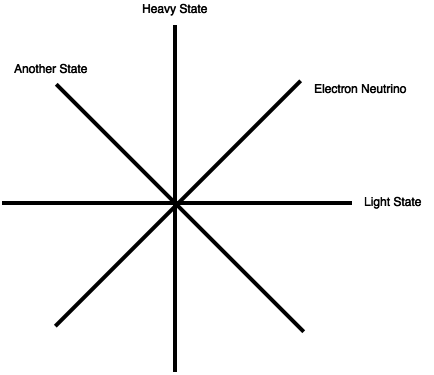
\includegraphics{assets/heavyLightRotation}
\caption{Due to this rotation, we can find an angle when the electron neutrinos becomes more important in Heavy state than Light state, which is $\theta=\frac{\pi}{4}$. For a mixing that has a larger angle, electron neutrinos actually take part in heavy neutrino state.}
\end{marginfigure}


\begin{align*}
\begin{pmatrix} \ket{\nu_L(x)} \\ \ket{\nu_H(x)} \end{pmatrix} &= \begin{pmatrix} \cos \theta(x) & -\sin\theta(x) \\ \sin\theta(x) & \cos\theta(x) \end{pmatrix} \begin{pmatrix}\ket{\nu_e} \\ \ket{\nu_x} \end{pmatrix} \\
& = \mathbf{U^{-1}_x } \begin{pmatrix}\ket{\nu_e} \\ \ket{\nu_x} \end{pmatrix} .
\end{align*}



To diagonalize it, we need to multiply on both sides the rotation matrix and its inverse, as we have done in the vacuum case,


\begin{equation}
\mathbf {H_{xd}} = \mathbf{U_x^{-1}} \mathbf H \mathbf {U_x}.
\end{equation}

The second step is to set the off diagonal elements to zero. By solving the equations we can find the  $\sin 2\theta(x)$ and  $\cos 2\theta(x)$ . \footnote{Just remember that $\Delta = \sqrt{2}G_F n(x)$ is a function of position.}

\begin{align*}
\mathbf{H_{xd}} &= \mathbf{U^{-1}_x} \left( A_1 \mathbf{ \sigma_1 } + A_3 \mathbf{\sigma_3} \right) \mathbf{ U_x } \\
& = \begin{pmatrix} A_3\cos 2\theta(x) - A_1 \sin 2\theta(x) & A_3 \sin 2\theta(x) + A_1 \cos 2\theta(x) \\ A_3 \sin 2\theta(x) + A_1\cos 2\theta(x) &  - A_3 \cos 2\theta(x) + A_1 \sin 2\theta(x) \end{pmatrix},
\end{align*}

where

\begin{align*}
A_3 &  = \frac{\Delta}{2} - \frac{\delta^2 m}{4E}\cos 2\theta_v \\
A_1 & =  \frac{\delta^2 m}{4E} \sin 2\theta_v.
\end{align*}

Set the off-diagonal elements to zero,

\begin{equation*}
A_3 \sin 2\theta(x) + A_1 \cos 2\theta(x)  = 0
\end{equation*}

So the solutions are

\begin{align*}
\sin 2\theta(x) & = \frac{A_1}{\sqrt{A_1^2 + A_3^2}} \\
\cos 2\theta(x) & = \frac{-A_3}{\sqrt{A_1^2+A_3^2}}.
\end{align*}

This diagonalizes the Hamiltonian LOCALLY. \footnote{The point is, for equation of motion, we have a differentiation with respect to position  $x$ ! So even we diagonalize the Hamiltonian, the equation of motion won't be diagonalized. An extra matrix will occur on the LHS and revert the diagonalization the Hamiltonian on RHS.
} It's not possible to diagonalize the Hamiltonian globally if the electron number density is not a constant.



As  $\Delta \to \infty$ ,  we have $A_3\to \infty$ and  $\sin 2\theta(x)$ vanishes. Thus the neutrino will stay on the defined light and heavy eigenstates if the interaction with matter is much larger than the vacuum energy. On the other hand, $\Delta \to 0$, everything gets back to the vacuum case.

Now we can obtain an approximate solution by using this approximate diagonalization. This idea is

\begin{equation*}
i \partial_x \Psi_x(x) = \mathbf{Extra Matrix From LHS}\cdot \mathbf H_{xd} \Psi_x(x),
\end{equation*}

where the $\mathbf{Extra Matrix From LHS}$ comes from the fact that changing from flavor basis $\Psi(x)$ to heavy-light basis $\Psi_x(x)$ using $\mathbf {U_x}$

\begin{equation*}
i\partial_x (\mathbf{U_x} \Psi_x(x)) = H ( \mathbf{U_x} \Psi_x(x) )
\end{equation*}

only returns

\begin{equation*}
i\partial_x \Psi_x(x) = \mathbf{H_{xd} } \Psi_x(x) - i \mathbf{U_x^{-1}} ( \partial_x \mathbf{U_x} ) \Psi_x(x).
\end{equation*}

Combining the two terms on RHS,

\begin{equation*}
i\partial_x \Psi_x(x) = \mathbf{H_x} \Psi_x(x),
\end{equation*}

where 

\begin{equation*}
\mathbf{H_x} = \mathbf{H_{xd}} - i \mathbf{U_x^{-1}} ( \partial_x \mathbf{U_x} ).
\end{equation*}

The only part inside $\mathbf{U_x(x)}$ that is space dependent is the number density of the electrons $n(x)$. {\bf{Thus we know immediately that the Hamiltonian is diagonalized if the number density is constant.}} \footnote{But even the electrons density is constant, the oscillation is different.}


%% As we said before, % I forgot what was that.

\subsection{Solar Density Profile}


The solar density profile can be determined using simple gravitational theory and nuclear physics models.

The mass contained in a spherical shell $dr$ is

\begin{equation}
    dm = 4\pi r \rho dr ,
\end{equation}

which is assuming spherical symmetry.

The gravitational potential for each unit of mass can generate force as gravitational attraction, which is

\begin{equation*}
    \frac{dv}{dr} = \frac{G m}{^2}.
\end{equation*}

The balance between pressure and gravity shows that

\begin{equation*}
    \frac{dv}{dr} \rho + \frac{dp}{dr} = 0.
\end{equation*}

The result of these relations is a rather intuitive relation between density and pressure, which is not solvable until we find another relation between them.

\begin{equation*}
    \frac{1}{r^2} \frac{d}{dr} \left( \frac{r^2}{\rho} \frac{dp}{dr} \right) = -4\pi G\rho.
\end{equation*}

To be simple, we will use Eddington model to solve the density profile, which gives us the relation

\begin{equation*}
    p = K \rho^{4/3},
\end{equation*}


where 
\begin{equation*}
    K = \left(  \left( \frac{k}{m_p} \frac{3}{\alpha} \frac{\beta}{\mu^4(1-\beta)^4}  \right)^4  \right)^{1/3}.
\end{equation*}

Combining the two relations between density and pressure, we can find the density profile with respect to radius.

By solving the equation, we get

\begin{equation*}
\frac{d\rho}{dr} = -\rho - \frac{3\pi G}{K} \rho^{8/3}.
\end{equation*}







\end{document}
